\chapter{Lösungen der Übungsaufgaben}

\structhead{Aufgabe 1.1.1.2:}
a) Zu der linearen Gleichung $6x_1 + 12x_2 = -6$ gehört folgende Gerade:

\begin{center}
  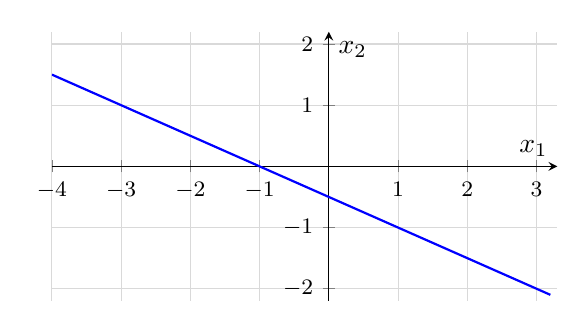
\begin{tikzpicture}
    \begin{axis}[width=8cm, height=5cm, axis lines=middle, xmin=-4, xmax=3.3, ymin=-2.2, ymax=2.2,
      xtick={-4,...,3}, ytick={-2,-1,1,2}, xlabel={$x_1$}, ylabel={$x_2$}, tick label style={font=\footnotesize}, samples=50, grid=both, grid style={gray!30}]
      \addplot[blue, thick, domain=-4:3.2] {-0.5*x-0.5};
    \end{axis}
  \end{tikzpicture}
\end{center}

Beispielsweise erfüllen folgende Wertepaare die Gleichung:
\[ \begin{pmatrix} x_1 \\ x_2 \end{pmatrix} = \begin{pmatrix} -3 \\ 1 \end{pmatrix}, \quad \begin{pmatrix} -1 \\ 0 \end{pmatrix}, \quad \begin{pmatrix} 0 \\ -\tfrac{1}{2} \end{pmatrix}, \quad \begin{pmatrix} 1 \\ -1 \end{pmatrix}, \quad \begin{pmatrix} \tfrac{3}{2} \\ -\tfrac{5}{4} \end{pmatrix}, \quad \begin{pmatrix} 2 \\ -\tfrac{3}{2} \end{pmatrix} \]
Alle Lösungen erhält man, wenn zu jedem $x_1$ der Wert von $x_2$ berechnet wird: $x_2 = -\tfrac{1}{2}x_1 - \tfrac{1}{2}$, also
\[ \begin{pmatrix} x_1 \\ x_2 \end{pmatrix} = \begin{pmatrix} x_1 \\ -\tfrac{1}{2}x_1 - \tfrac{1}{2} \end{pmatrix} . \]

b) Folgende Möglichkeiten gibt es:
\begin{itemize}
  \item Alle drei Geraden sind identisch: Es gibt unendlich viele Lösungen.
  \item Zwei Geraden sind identisch, die dritte schneidet sie: Es gibt genau eine Lösung.
  \item Alle drei Geraden sind parallel zueinander: Es gibt keine Lösung.
  \item Zwei Geraden sind parallel, die dritte Gerade schneidet sie in verschiedenen Punkten: Es gibt keine Lösung (Bild 1).
  \item Alle drei Geraden schneiden sich in einem Punkt: Es gibt genau eine Lösung (Bild 2).
  \item Die drei Geraden schneiden sich in drei verschiedenen Punkten. Also gibt es keine Lösung (Bild 3).
\end{itemize}

\structhead{Aufgabe 1.1.1.4:}
a) Die Matrix lautet:
\[ (A\,|\,b) = \left(\begin{array}{cccc|c} 3 & 0 & 4 & -2 & 0\\ 0 & -1 & 1 & 1 & 0{,}5\\ 0 & 0 & 1 & 0 & 12 \end{array}\right) \]
b) Das LGS lautet:
\begin{align*}
  x_1 + 2x_2 &= 5\\
  x_2 + 3x_3 &= 12\\
  -x_1 + x_3 &= -8
\end{align*}

\structhead{Aufgabe 1.2.1.4:}
a) Die Matrix
\[ \left(\begin{array}{ccc|c} 1 & 0 & 0 & 2\\ 0 & 1 & 0 & 3\\ 0 & 0 & 1 & -2 \end{array}\right) \]
liefert die Lösung $\vec{x} = \begin{pmatrix} 2 \\ 3 \\ -2 \end{pmatrix}$.

b) Die Matrix
\[ \left(\begin{array}{ccccc|c} 1 & 0 & 3 & 0 & 0 & 2\\ 0 & 1 & 0 & 0 & 0 & -2\\ 0 & 0 & 0 & 1 & 0 & 0\\ 0 & 0 & 0 & 0 & 1 & 2 \end{array}\right) \]
führt zu den Lösungen
\[ \begin{pmatrix} x_1 \\ x_2 \\ x_3 \\ x_4 \\ x_5 \end{pmatrix} = \begin{pmatrix} 2 - 3x_3 \\ -2 \\ x_3 \\ 0 \\ 2 \end{pmatrix} . \]

\structhead{Aufgabe 1.4.1.1:}
Es gilt:
\[ 5 \cdot \begin{pmatrix} 0 & 0 & 3 & -6 \\ 0 & 1 & 0 & 3 \\ 1 & 1 & 0 & 5 \end{pmatrix} = \begin{pmatrix} 0 & 0 & 15 & -30 \\ 0 & 5 & 0 & 15 \\ 5 & 5 & 0 & 25 \end{pmatrix}, \qquad 3x \cdot \begin{pmatrix} 6 & 0 \\ 0 & 2 \\ 4 & 1 \end{pmatrix} = \begin{pmatrix} 18x & 0 \\ 0 & 6x \\ 12x & 3x \end{pmatrix} \]
b) $\vec{v} + \vec{w} = \begin{pmatrix} 2 \\ 0{,}5 \\ -0{,}3 \end{pmatrix} + \begin{pmatrix} -1 \\ 0 \\ 0{,}7 \end{pmatrix} = \begin{pmatrix} 1 \\ 0{,}5 \\ 0{,}4 \end{pmatrix}$

c) $\begin{pmatrix} 2 \\ 0 \\ 1 \\ 8 \end{pmatrix} + \begin{pmatrix} x \\ 0 \\ 2x \\ -3 \end{pmatrix} = \begin{pmatrix} 2 + x \\ 0 \\ 1 + 2x \\ 5 \end{pmatrix}$

\structhead{Aufgabe 1.4.1.4:}
\[ A \cdot \vec{b} = \begin{pmatrix} 13 \\ 29 \end{pmatrix}, \qquad A \cdot C = \begin{pmatrix} 1 & 2 & 12 \\ 3 & 4 & 24 \end{pmatrix}, \qquad C \cdot D = \begin{pmatrix} 2 & 0 & 1 \\ 6 & 1 & 9 \end{pmatrix}, \qquad D \cdot F = \begin{pmatrix} 1 & 0 & 4 \\ 0 & 1 & 0 \\ 0 & 0 & 3 \end{pmatrix} \]

\structhead{Aufgabe 2.1.1.1:}
Das Lösungsgebiet ist in der folgenden Abbildung schraffiert dargestellt.

\begin{center}
  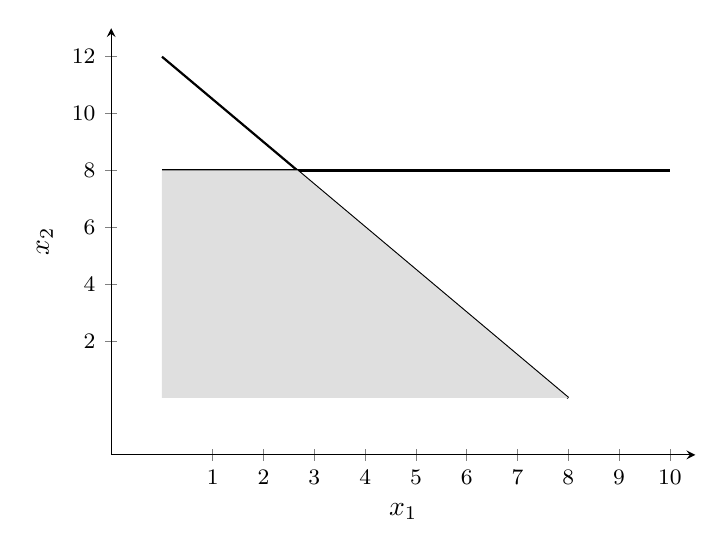
\begin{tikzpicture}
    \begin{axis}[width=9cm, height=7cm, axis lines=left, xmin=-1, xmax=10.5, ymin=-2, ymax=13,
      xtick={1,...,10}, ytick={2,4,...,12}, xlabel={$x_1$}, ylabel={$x_2$}, tick label style={font=\footnotesize}, samples=50, clip=true]
      \addplot[black, thick, domain=0:8] {12-1.5*x};
      \addplot[black, thick, domain=0:10] {8};
      \fill[gray!25] (axis cs:0,0) -- (axis cs:0,8) -- (axis cs:2.667,8) -- (axis cs:8,0) -- cycle;
    \end{axis}
  \end{tikzpicture}
\end{center}

\structhead{Aufgabe 2.1.1.4:}
Im folgenden Bild sind für die drei $Z$-Werte 24, 28 und 32 die Isogewinngeraden eingezeichnet. Wie man sieht, »erwischt« die Gerade zu $Z = 32$ gerade noch den Eckpunkt mit $x_1 = 8$ und $x_2 = 0$, der maximale $Z$-Wert ist also 32.

\begin{center}
  \begin{tikzpicture}
    \begin{axis}[width=9cm, height=7cm, axis lines=left, xmin=-1, xmax=10, ymin=-1, ymax=35,
      xtick={1,...,8}, ytick={10,20,30}, xlabel={$x_1$}, ylabel={$x_2$}, tick label style={font=\footnotesize}, samples=50, clip=true]
      \addplot[black, thick, domain=0:8] {12-1.5*x};
      \addplot[black, thick, domain=0:10] {8};
      \addplot[dashed, domain=0:8] {24-4*x};
      \addplot[dotted, domain=0:8] {28-4*x};
      \addplot[dashed, thick, domain=0:8] {32-4*x};
      \node[above right] at (axis cs:6,4) {$Z=32$};
    \end{axis}
  \end{tikzpicture}
\end{center}
